%% LyX 2.1.3 created this file.  For more info, see http://www.lyx.org/.
%% Do not edit unless you really know what you are doing.
\documentclass[english]{article}
\usepackage[T1]{fontenc}
\usepackage{amssymb}
\usepackage{graphicx}
\usepackage{amsmath}
\usepackage{setspace}
\usepackage{babel}
\begin{document}
\begin{onehalfspace}

\title{Image Processing using Convolutional Neural Networks}
\end{onehalfspace}

\begin{onehalfspace}

\author{Teng Hu, Chengen Xie}
\end{onehalfspace}

\maketitle
\begin{onehalfspace}

\section{Abstract}
\end{onehalfspace}

\begin{onehalfspace}
Defining a specific artistic style has been a controversial topic in both arts and neural science field.  In the paper \textit{A Neural Algorithm of Artistic Style}. The authors introduce a approach  by using  an artificial system with deep neural network to applied existing art style from a input painting into a new painting.

Our approach is to learn and testify the model behind the paper and replicate the output. The algorithm captures the style information within different layers of the network, then construct the image that matches the style representation of the given input image. Initially we are planning to implement the algorithms and utilizing Caffe package to implement the convolution learning network. 

In addition, we tweak the model by implement new layers of learning network, analyze the correspondence between different loss functions and texture representation. 
\end{onehalfspace}


\begin{onehalfspace}
\section{Model Summary}
\end{onehalfspace}

\begin{onehalfspace}
Convolutional neural network is designed to take advantage of the 2D structure of images. CNN consists of a number of convolutional layers and follow by one or more fully connected layers as in standard multilayer neural network. One major benefit is that CNN is easier to train and have fewer parameters than fully connected networks with the same number of hidden units. 

CNN is a special kind of neural network have layers of feature maps which consist of small filters per layer. What CNN does in one layer is apply the filter on input image(representation) and output a layers of data, which is a higher level representation of the original input.
CNN convolve several filters on the input image, also subsample the original one to smaller pieces of images, repeatedly layer by layer. In the mathematical context, convolution is defined as applying a function across the output of another function. In Image processing , applying convolution means applying a filter over the image at all offsets to extract certain information, e.g. mean filtering,  neighborhood-averaging filtering and edge detection. 

\newline
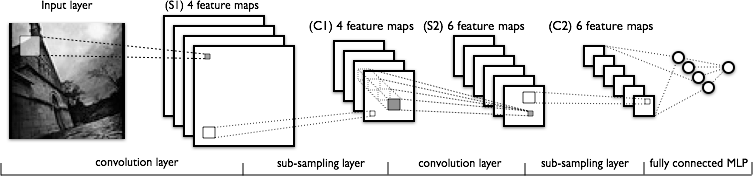
\includegraphics[width = \textwidth]{image3}
\newline


The model in the paper is using VGG Network. First it abstract the content from original image. It noted that p is the original image, and x is the generated image, l is the layer. In each layer in CNN, x is encoded by the filter. The loss function can be written as following:
\begin{center}
$L_{content}(\vec{p},\vec{x},l)=\frac{1}{2}\sum_{i,j}(F^l_{ij}-P^l_{ij})^2$
\end{center}

It can be derived as:
\begin{center}
$\frac{\partial L_{content}}{\partial F^l_{ij}}=\left\{
    \begin{array}{lr}
     (F^l-P^l)_{ij} & if F^l_{ij}>0\\
     0 & if F^l_{ij}<0
     \end{array}
    \right.$
\end{center}

The input x will change until it converge in the output in a certain layer of the CNN as p. The model also computes the correlation between different filter response above CNN in each layer. As represented by:
\begin{center}
$G^l_{ij}=\sum_{k}F^l_{ik}F^l_{jk}$
\end{center}

To generate texture, the model uses gradient descent from white noise.
In order to mix the image with art style, the model will minimize the distance of a white noise image to match the art style. The total loss function is
\begin{center}
$E_l=\frac{1}{4N^2_lM^2_l}\sum_{ij}(G^l_{ij}-A^l_{ij})^2$
\end{center}
\begin{center}
$L_{style}(\vec{\alpha},\vec{x})=\sum_{l=0}^{L}w_lE_l$
\end{center}


To generate the image using the texture the model minimizes the loss function of distance of white noise of the picture and the style from different CNN layers.
\begin{center}
$L_{total}(\vec{p},\vec{\alpha},\vec{x})=\alpha L_{content}(\vec{p},\vec{x})+\beta L_{style}(\vec{\alpha},\vec{x})$
\end{center}

\end{onehalfspace}

\begin{onehalfspace}
\section{Image Process Result}
\end{onehalfspace}

\begin{onehalfspace}
We successful generated the similar output as the author mentioned in the paper with 100 to 1000 iterations.


\end{onehalfspace}


\end{onehalfspace}

\begin{onehalfspace}
\section{Further Improvement}
\end{onehalfspace}

\begin{onehalfspace}
Thereare various optimization for CNN with different advantages and
disadvantages. For example, stochastic gradient descent(SGD), LBFGS,
Limited memory BFGS and Conjugate gradient. SGD is easy to implement,
and very fast when there are enough training set, however, SGD
requires us to set parameter manually, like learning rate,
convergence condition. It is proved in paper \textit{On Optimization
Methods for Deep Learning} that among all
methods, LBFGS is highly desirable for convolution models. Conjugate
gradient is more competitive in high dimensional problems compare to
LBFGS and SGD.

For our experiment, we could use LBFGS as our optimization method of the
algorithm. The algorithm currently runs very relatively on PC (it takes
about an hour to finish 1000 iterations). However, there are
sophisticated algorithms designed to optimize the algorithm, we can
improve the optimization by using Bayesian methods. For example, adding
the proper amount of noise to the gradient optimization algorithm
could turn the optimization more likely converge to the samples from
the posterior distribution. As we proposed, in the future, we may
test the results with SGD,  compare the results with LBFGS, and add
Gaussian noise to the LBFGS/ADAM in further investigation.  

\end{onehalfspace}

\begin{onehalfspace}
\section{Conclusion}
\end{onehalfspace}

\begin{onehalfspace}
In our project we studied and implemented the model in A Neural Algorithm of Artistic Style, using Torch 7 and VGG-network model in caffe.

It is well-known that Convolutional Neural Networks are very powerful in Image Processing and already have many interesting applications. The reasons lie in the structure of CNN. Convolutional Neural Networks consist of layers of computational units that process information through feedforward propagation. Each layer of units is a collection of image filters and extracts a different feature of the image. In this paper, the major finding is that the representations of content and style in CNN�
can be separable in layers to some extent, thus we can extract the style of the picture and use it to produce new one combined with other content. In brief, the content of the image we are looking at is referred to positions and arrangement of objects which are stored in high level layers when CNN is trained for object recognition, for the same reason, we can recognize these output images originates from one same image, because our brain recognizes the object unconsciously. On the other hand, the algorithm uses a feature space to store texture information. The feature space consists of correlations between the different filter responses in each layer of network. We extract the style of image by including feature correlations of multiple layers.


\end{onehalfspace}


\begin{thebibliography}{9}
\bibitem{1} 
Simonyan, K. and Zisserman, A.
Very Deep Convolutional Networks for Large-Scale Image Recognition,CoRR, abs/1409.1556, 
 
 \bibitem{2} 
Leon A. Gatys, Alexander S. Ecker, Matthias Bethge
A Neural Algorithm of Artistic Style

\bibitem{2} 
neural-style
\\\texttt{https://github.com/jcjohnson/neural-style}

\bibitem{2} 
CNN image
\\\texttt{http://deeplearning.net/tutorial/_images/mylenet.png}


\end{thebibliography}
\end{onehalfspace}
\end{document}

